\chapter{Introduction}
Computer scientists continue to gain influence in our society. Greater influence
means that large corporations and government bodies are funding and supporting
computer engineers for development of the world’s newest technologies. Computers
manage increasingly many aspects of our lives, and we still have not tapped their full
potential. Still, there is no specific body, and few rules in place to assure that computer
program technologies will be safe and beneficial to the general public. Artificial
intelligence (AI) is now becoming a reality, and no one knows for sure what direction it
will take. In light of new developments in intelligent programming technologies like
neural networking, this paper will argue that truly intelligent machines may be in our
future. More importantly, it will establish that computer scientists have considerable
ethical and political responsibilities to the public.


\section{What is Artificial Intelligence}

Artificial intelligence is the design and study of computer programs that behave
intelligently \cite{one}. It is in many ways the ultimate goal of computer programming.
There is an ongoing effort to make more intelligent computer programs that are easier to
use, even at the expense of simplicity and efficiency. Programs, after all, are designed to
solve problems. That they should do so intelligently is a logical objective. This chapter
will explain what it means for a computer program to behave intelligently and outline
some uses for intelligent programs.

    \subsection{Recognizing Artificial Intelligence}
    
    It is difficult to define exactly what we mean when saying that a computer
program should behave intelligently. Most people can give an abstract definition of
intelligence, and anyone can look it up in a dictionary. However, conventional
definitions of intelligence, like many commonly used expressions, are too ambiguous to
be directly and usefully applied to computers. It is impossible to describe artificial
intelligence, or to gauge our progress in that field, without knowing how intelligence
applies to computers.\\
In a paper in 1950, Alan Turing proposed a test to measure the intelligence of
computer programs \cite{two}. Turing refers to this test as the ‘imitation game’ (though
it has since been dubbed simply the Turing test). In the imitation game, a human judge
uses a Teletype or some other simple interface to interrogate both a man (A) and a
woman (B). The interrogator does not know in advance whether A is male and B is
female, or vice versa. It is A’s job to convince the interrogator that A is actually a
woman. If asked, for example, the length of his hair, A might indicate that it is straight
and layered, with the longest strands being several inches. It is B’s job to help the
interrogator figure out which interrogatee is male and which is female. B might type
things like, \say{I am the woman! Trust me!} Such statements, however, would be of
limited value, since A could easily type the same.\\

\begin{figure}[H]
    \centering
    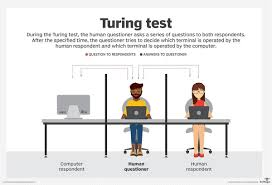
\includegraphics{images/turing.jpg}
    \caption{Turing test}
    \source{Source: https://www.techopedia.com/definition/200/turing-test}
    \label{fig:my_label}
\end{figure}

Roughly half of the time, the interrogator might be fooled into believing that A is
actually the woman. Suppose, however, that A were a computer rather than a man. If
that computer could win the imitation game, i.e. fool the human interrogator, with the same frequency as a man, then the computer is said to have passed the Turing test. In
terms of Turing’s original paper, the computer might be judged capable of thinking.\\
While passing of the Turing test implies some definition of artificial intelligence,
it is insufficient for describing modern AI systems. As computer science has begun to
mature, we have developed new goals and uses for artificial intelligence, as well as new
technologies for achieving those goals. Intelligent systems need not be designed to fool a
human judge. Nor is such a facade necessarily desirable. A human working in a factory,
for example, would require rest, supervision, and incentive to continue working. These
are not characteristics we choose to emulate in computer programs. Yet there seems to
be something intelligent about a robotic system that can, for example, build or design
cars.\\
It is perhaps better to think of artificial intelligence as the study and design of
computer programs that respond flexibly in unanticipated situations \cite{one}. A
computer program can give the illusion of intelligence if it is designed to react sensibly to
a large number of likely and unlikely situations. This is similar to the way we might
judge human intelligence, by a person’s ability to solve problems and cope effectively
with a wide variety of situations \cite{three}. In this case, it is not necessary for an intelligent
program (or person) to develop an original solution to a problem.\\
Still, to say that a computer program should react sensibly to situations is
analogous to saying that it should react intelligently. In other words, the meaning of
intelligence in terms of computers remains elusive. For the purposes of this paper, we
will say that artificial intelligence is defined by two major methodologies and their
purposes. Weak artificial intelligence is the design of computer programs with the intention of adding functionality while decreasing user intervention. Many modern word
processors are designed to indicate misspelled words without being asked to do so by the
user. Some programs will even correct misspellings automatically. This is an example of
weak artificial intelligence.\\
Strong artificial intelligence is the design of a computer program that may be
considered a self-contained intelligence (or intelligent entity). The intelligence of these
programs is defined more in terms of human thought. They are designed to think in the
same way that people think. Passage of the Turing test, for example, might be one
criterion for development of a strong AI system. The ethical issues in this paper deal
largely with the strong AI methodology. However, the bulk of useful artificial
intelligence applications lie in the realm of weak AI.
    
    \subsection{Applications of Artificial Intelligence}

    Artificial intelligence is useful in many domains, and its reach is constantly
growing. The first step in artificial intelligence programming is automated reasoning.
Automated reasoning is a computation that takes some encoded knowledge about the
world as input and provides inferred conclusions based on that knowledge as output
\cite{four}. In the beginning, this automated reasoning programming was merely
academic. Today, automated reasoning is used in video games, air traffic control
systems, and the Mars rover.
Clearly, some of these programs require skills that we might normally associate
with natural intelligence. Some things seem quite simple, like driving around a sandy
planet surface. Nonetheless they are all useful, and they represent what we consider to be
intelligent computer programs. There seem to be, however, many more things that we want computers to do for us. Research continues as we stretch the limitations of
computing devices, challenge each other to create greater intelligence sys tems, and
struggle to define computer intelligence.

\section{Limitations of Artificial Intelligence}
    
    Computer power continues to increase exponentially. This refers both to the
speed of computing devices and the influence they have over our lives. Moore’s Law
predicts that computers will double in speed and halve in size every eighteen months
\cite{five}. While this law has held for over 35 years, current trends suggest that
engineers will someday be limited by the sizes of molecules used in the construction of
integrated circuits. Growth of computer power is linked growth of artificial intelligence
systems. What, then, are the limitations of AI?\\
There are some computer programs that create original paintings from brushstroking
rules and stored images of objects. There are others that generate sensible haiku
poetry from lists of related words (Kurzweil 163-9). These programs might be said to
have passed a simplified and artistic variation of the Turing test. They demand some
consideration when talking about artificial intelligence, but, given that they simply follow
expansive sets of rules, how intelligent are they? There is some question, for example, as
to whether a computer-generated poem can really be art. In these cases, and most cases
of AI development, intelligent behavior boils down to a search over some set of possible
actions and outcomes.
There have been lengthy debates over the limits of computer intelligence. Surely
we can rely on the fact that computers will continue to get more powerful, and thus able to perform more tasks in less time. Still, there may be things that a computer could never
do. Specifically, it is unclear whether any product of the strong artificial intelligence
methodology will ever succeed. That is, it is unclear whether a computer program will
ever constitute a mind.
    \subsection{The Chinese Room}

    During the mid 1960’s and through the 1970’s, academic institutions and
individuals put a great deal of effort into the research and development of strong artificial
intelligence. One such project, developed at Yale University by Roger Schank and his
colleagues, was designed to answer various questions about predetermined material
\cite{six}. (Today these programs are called expert systems.) Some argued that
these projects were the beginnings of strong AI. In response to such claims, Philosopher
John Searle wrote a classic proposition commonly called the “Chinese Room” example to
refute this claim \cite{six}. The example was not only meant to demonstrate that strong AI
was not a reality, but that no Turing machine could produce a strong artificial
intelligence.\\
In Searle’s example, he is locked in a room with a stack of Chinese symbols.
Searle speaks no Chinese, and could just as well be locked in a room with a stack of
meaningless squiggles. A second stack of squiggles is introduced, along with instructions
showing how to correlate the first stack of symbols with the second stack. The
instructions are in English, which Searle understands perfectly, and they allow him to
correlate the Chinese symbols entirely by their shapes. That is to say that the semantics
of the symbols remain unknown to Searle. People outside the room are allowed to send
more stacks of Chinese symbols under the door. When Searle receives these stacks, he reads in his instructions how to correlate the old symbols with the new ones. He is then
able to send back an appropriate stack of squiggles according to his instructions.\\

\begin{figure}[H]
    \centering
    
\includegraphics{images/chinese.jpg}
    \caption{Chinese Room Argument}
    \source{Source: https://www.iep.utm.edu/chineser/}
    \label{fig:my_label}
\end{figure}

Searle argues that with a large enough set of instructions, he could fool anyone
into thinking that he knew Chinese. Yet he clearly does not know Chinese. Similarly,
computers that answer questions about predetermined material do not understand that
material. They simply manipulate sets of formal symbols according to instructions in
their native language. Searle’s example is immensely more complex, however, in the
sense that the Chinese room is designed to handle any reasonable domain of knowledge
that a Chinese person might ask about.\\
The Chinese room is really only a philosophical version of the Turing test,
passage of which is likely to be insufficient for defining strong artificial intelligence.
Moreover, Searle points out that he could fool anyone into thinking that he was Chinese.
This means that Searle must have an uncountable number of symbol correlations, because
he must account for previous conversations and answer compounding inquiries
appropriately. Regardless of whether Searle knows what he is doing, something about
the Chinese room must understand Chinese. To say that Searle does not understand
Chinese is analogous to saying that my mouth does not understand English. The
understanding is contained in the set of instructions. While there may be no metaphysical
understanding, it seems that if Searle and the room can correlate intelligible symbols
about any subject, I might say that they (they as an entity) were intelligent. Moreover,
the constant addition of new instructions is directly analogous to learning, another
seemingly intelligent trait.\\
Searle’s example does raise, however indirectly, the question of tractability. The
fact that something is possible in theory does not make it a reasonable undertaking. To
build a computer program like the Chinese room (in the same way that Searle describes
it) one would require almost infinite memory and constantly increasing computational
power. The Chinese Room example shows, in part, why strong AI is so elusive. Imagine
the sheer size of the translator’s book if he could handle all possible sensible
combinations of Chinese symbols. The human brain is constantly bombarded with input
from the five senses and somehow manages it all. We simply lack the technology and
understanding to replicate that type of behavior at present. Moreover, the human mind
may be more than just the sum of its parts. This idea, called dualism or the mind-body
problem, is another roadblock to the understanding of computer-based intelligence.


\section{Ethical Issues}
On a philosophical level, there are important moral issues facing the developers of
strong AI sys tems. Given that the goal is to develop an independently intelligent
computer program, we should consider briefly how to classify such an entity. A strong
artificial intelligence would surely call into question (for some) that which we define as
“alive.” It is yet unclear whether an intelligent electronic entity would be alive and
legally entitled to certain rights.\\
There is no evidence that intelligent life, as it applies to human- like intelligence,
is sustainable without a soul. Nor is there evidence that a soul is necessary. In fact, there
is no complete definition of a soul at all. For some it is a vehicle by which we relate to a
higher power, and for others it is nothing but nonsense. We must therefore consider questions pertaining to life and intelligence notwithstanding the existence or nonexistence
of a soul. In that case, it is impossible to say whether an entity inside a computer would
be alive. However, there is more than enough uncertainty to say that such consideration
must be given. There is no accounting for science, and it is impossible to tell exactly
what questions future science will answer. In science, therefore, the case of moral
justification must not be taken in terms of what will happen, but in terms of what might
happen \cite{seven}. An intelligent entity within a machine would likely have a justifiable
claim to legal and possibly even civil rights, and pulling the plug on that machine may
well constitute negligent or malicious killing.\\
With regard to the metaphysical problem of a soul, many people in the world
believe that souls exist, and that all intelligent creatures have souls. In Kenneth
Branagh’s 1994 cinematic adaptation, Mary Shelley’s Frankenstein, Frankenstein’s fiend
asks of his creator, “What of my soul? Do I have one?” A reasonably intelligent
computer entity may be compelled to ask the same questions. An independently thinking
entity certainly might have rights to those answers. How would the AI programmers
respond to such inquiries? For some it is not simply a question of whether computer
programs can have souls, but a question of who would be willing to take responsibility
for those souls.\\
The remainder of this paper introduces arguments that strong artificial intelligence
systems may be in our future. As the introduction of intelligent systems would almost
certainly change our world in a dramatic way, the paper will then discuss several possible
futures involving artificially intelligent machines. At its conclusion, the paper will show
that computer scientists have the ultimate responsibility in making their products as safe as possible. The lack of a strictly enforced regulatory standard on software development
means that computer scientists must exercise independent self-governance when
developing controversial and unpredictable technologies such as artificial intelligence
networks. This responsibility, however, should not fall solely on programmers. The
paper will bring to light the necessity for trained engineers to be more intimately involved
in managerial and political positions.



